\documentclass{article}

\usepackage{listings}
\usepackage{multicol}
\usepackage{tikz}
\usepackage{fancyhdr} % Fancy headers and footers
\usepackage{amsthm, amsmath, amsfonts, amssymb, mathrsfs, mathtools} % Math packages
\usepackage{enumitem}
\usepackage{geometry}
\usepackage{marginnote}

%% For inkspace figures:
\usepackage{import}
\usepackage{xifthen}
\usepackage{pdfpages}
\usepackage{transparent}
\newcommand{\incfig}[1]{%
    \def\svgwidth{\columnwidth}
    \import{./figures/}{#1.pdf_tex}
}
\pdfsuppresswarningpagegroup=1

%% Set document margin:
\geometry{margin=1in} %% Add paperheight=16383pt to make page continuous


\newtheorem{theorem}{Theorem}[section]
\newtheorem{corollary}{Corollary}[theorem]
\newtheorem{lemma}[theorem]{Lemma}
\newtheorem*{remark}{Remark}
\theoremstyle{definition}
\newtheorem{definition}{Definition}[section]

\newtheoremstyle{note}{3pt}{3pt}{\normalfont}{}{\bfseries}{:}{ }{}
\theoremstyle{note}
\newtheorem*{note}{Note}

%% Margin Notes
\let\oldmarginpar\marginpar
\renewcommand{\marginpar}[2][text width=3cm, rectangle, draw,rounded corners, thick]{%
        \oldmarginpar{%
        \tikz \node at (0,0) [#1]{#2};}%
        }


%% Header and Footer
\pagestyle{fancy}
\fancyhf{}
\lhead{\classname} % Left Header text
\rhead{} % Right header text
\rfoot{Page \thepage}


%%% ADD OPTIONAL HEADER AND FOOTER RULES

%%% CHANGE SNIPPETS _ AND ^ TO DETECT IF
%%% {} HAVE ALREADY BEEN WRITTEN


%%% INPUTS %%%%%%%%%%%%%%%%%%%%%%%%%%%%%%%%%%%
\newcommand{\classname}{Project Notes}


%%% SNIPPET COMMANDS %%%%%%%%%%%%%%%%%%%%%%%%%%%%%%%%%%%%%


%%%%%%%%%%%%%%%%%%%%%%%%%%%%%%%% Random stuff
% ital - \textit{}
% bld - \textbf{}
% margin - \marginnote{text}[offset]

%%%%%%%%%%%%%%%%%%%%%%%%%%%%%%%% Random math stuff
% dx  - \frac{\\partial $1}{\\partial $2}
% rarrow - \\rightarrow
% func - \\$1 : \\mathbb{$2} \\rightarrow \\mathbb{$3}, x \\mapsto 
% txt - \text{$1}
% // - \\frac{$1}{$2}$0
% sum -  \\sum \\limits $0
% qed - qed symbol (filled)
% inv - inverse ^{-1}
% mmath - $ input $ 

%%%%%%%%%%%%%%%%%%%%%%%%%%%%%%%% Environments
% align - \begin{alignedat}{4}
% props - \align{} - Numbered
% bm - \\begin{bmatrix} $1 \\end{bmatrix}
% pm - \\begin{pmatrix} $1 \\end{pmatrix}
% thm - \\begin{thm}{$1} $1 \end{thm}
% def - \\begin{def}{$1} $1 \end{def}
% lemma - \begin{lemma}
% cor - corollary \begin{corollary}
% proof - \begin{proof}
% remark - \begin{remark}
% dm -  \[\]
% beg - \begin{$1} \end{$1}
% python - \begin{lstlisting}[language=Python,escapeinside={(*}{*)}, basicstyle=\fontsize{11}{13}]
% section -  \section{}
% subsection -  \subsection{}

%%%%%%%%%%%%%%%%%%%%%%%%%%%%%%%% Constants
% reals - \mathbb{R}
% rationals - \mathbb{Q}
% integers - \mathbb{Z}
% complex - \mathbb{C}
% eps -  \\epsilon
% sig - \\sigma
% Sig - \\Sigma
% prime - ^{\prime}
% alpha - \\alpha
% beta - \\beta



%%%% START OF DOCUMENT ############
\begin{document}


\section{How does Spot actually work?}
\begin{figure}[ht]
    \centering
    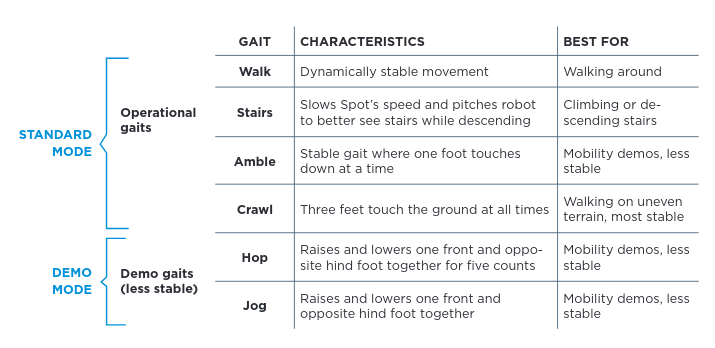
\includegraphics[scale=0.4]{./figures/screenshot.png}
\end{figure}
\begin{figure}[ht]
    \centering
    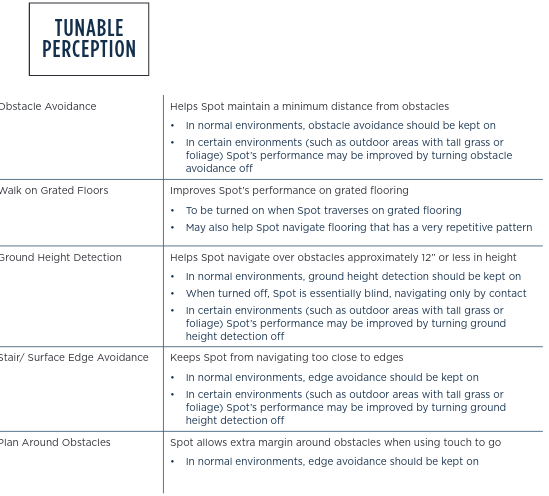
\includegraphics[scale=0.4]{./figures/screenshot2.png}
\end{figure}
Spot has the user specify gaits before hand. Using the wrong gait for the task means spot can fall.



\section{Paper Notes}
\subsection{Automatic  Gait  Pattern  Selection for  Legged  Robots}
\begin{itemize}
    \item Model the robot as a single rigid body along with $ n_ {l} $ mass-less legs.
\end{itemize}
\subsubsection{Problem Description:}

\begin{itemize}
    \item $ \tau = [r, \Theta]^ {T} $
        \begin{itemize}
            \item Where $ r \in \mathbb{R}^ {3}$ is Center of Mass(CoM) position    
            \item $ \Theta \in \mathbb{R}^ {3} $ is yaw, pitch, and roll angles
        \end{itemize}
    \item 
\end{itemize}



\subsection{Gait and Trajectory Optimization for Legged Systems Through Phase-Based End-Effector Parameterization}
%https://www.youtube.com/watch?v=KhWuLvb934g&feature=emb_logo
\subsubsection{Related Work}
\textbf{Commonality} with the following Dynamics models are that they all predefine some motion before hand.
\begin{itemize}
    \item \textit{Linear Inverted Pendulum model} (LIP) which only optimizes over the Center of Mass position.
    \begin{itemize}
        \item By modeling the robot as an inverted pendulum, the position of the Center of Pressure (CoP) or Zero-Moment Point(ZMP) can
        be used as a substitute for contact forces, and is used to control the motion of the Center of Mass. 
        \item Fast and pretty effective.
        \item BUT this method uses predefined footholds.
    \end{itemize}
    \item Another common model in Trajectory Optimization is the \textit{Centroidal Dynamics} model.
    \begin{itemize}
        \item Projects the effects of all link motions onto 6-dimensional base. 
        \item the input that drives this system are the contact forces, as opposed to the Center of Pressure in the Linear Inverted Pendulum or the 
        joint torques in the full rigid-body dynamics.
    \end{itemize}
\end{itemize}


\subsection{A Robust Quadruped Walking Gait for Traversing Rough Terrain}
\subsubsection{Things to Note:}
\begin{itemize}
\item "Obviously, a robust balancing  controller  is  the  prerequisite  for  legged  locomotion,  and it is usually characterized by a special control variable, for instance, the locations of the center-of-gravity (COG) in static walking, or the zero-moment-point (ZMP) in dynamic walking. "
\item In this paper  we  address  how  to  generate  a  robust  COG  trajectory  for  a  quadrupedal  walking  robot,  and  how  to  convert  this plan  into  an  appropriate  joint-space  walking  pattern.
\item They adjust the COG trajectory continuously in response to the current movement of the feet of the robot, in smooth twice differentially way.
\end{itemize}


\end{document}




